\newcommand{\halfangle}{10}
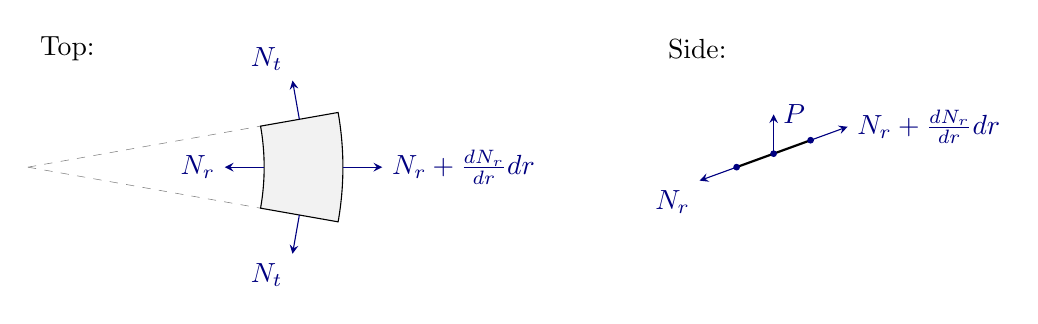
\begin{tikzpicture}[scale=2]
	%The radial equilibrium
	\begin{scope}[xshift=-4.5 cm]
		%The bisected dotted lines
		\begin{scope}[dashed,gray,very thin]
			\draw (0,0) -- (\halfangle:1.5 cm);
			\draw (0,0) -- (-\halfangle:1.5 cm);
		\end{scope}
		%Draw the area element
		\filldraw[fill=gray!10,draw=black] (-\halfangle:1.5 cm)  arc(-\halfangle:\halfangle:1.5 cm) -- (\halfangle:2 cm) arc(\halfangle:-\halfangle:2 cm) -- cycle;
		%Draw the force lines and labels
		\begin{scope}[->, blue!50!black,>=stealth]
			\draw (0:2 cm) -- +(0:.25 cm) node[anchor=west]{$N_r+\frac{dN_r}{dr} dr$};
			\draw (0:1.5 cm) -- +(0:-.25 cm) node[anchor=east]{$N_r$};
			\draw (\halfangle:1.75 cm) -- +(90+\halfangle:.25 cm) node[anchor=south east]{$N_t$};
			\draw (-\halfangle:1.75 cm) -- +(-90-\halfangle:.25 cm) node[anchor=north east]{$N_t$};
		\end{scope}
		\draw (.25,.75 cm) node{Top:};
	\end{scope}
	
	%The lateral equilibrium
	\begin{scope}[->, blue!50!black,>=stealth]
		\draw (0,0) -- (20:-.25 cm) node[anchor=north east]{$N_r$};
		\draw[black,thick,-] (20:0 cm) -- ++(20:.5 cm);
		\draw (20:.5 cm)  -- ++(20:.25 cm) node[anchor=west]{$N_r+\frac{dN_r}{dr} dr$};
		\draw (20:.25 cm) -- ++(90:.25 cm) node[anchor=west]{$P$};
		\filldraw (0,0) circle(.5pt);
		\filldraw (20:.5 cm) circle(.5pt);
		\filldraw (20:.25 cm) circle(.5pt);
	\end{scope}
	\draw (-.25,.75 cm) node{Side:};
	
\end{tikzpicture}